\documentclass[conference]{IEEEtran}
\IEEEoverridecommandlockouts
% The preceding line is only needed to identify funding in the first footnote. If that is unneeded, please comment it out.
\usepackage{cite}
\usepackage{amsmath,amssymb,amsfonts}
\usepackage{algorithmic}
\usepackage{graphicx}
\usepackage{textcomp}
\usepackage{xcolor}
\usepackage{tabularx}
\usepackage{multirow}
\usepackage{graphics} % for pdf, bitmapped graphics files
\usepackage{subfig}
\usepackage{subcaption}
\usepackage{hyperref}
\usepackage{academicons}
\usepackage{xcolor}
\usepackage{listings}
\def\BibTeX{{\rm B\kern-.05em{\sc i\kern-.025em b}\kern-.08em
		T\kern-.1667em\lower.7ex\hbox{E}\kern-.125emX}}
% Gráficas en MATLAB
\usepackage{tikz, pgfplots}
% Color Enlace
\definecolor{colorEnlace}{RGB}{0, 0, 0}
\hypersetup{
	colorlinks=true,
	linkcolor=colorEnlace,
	citecolor=colorEnlace,
	urlcolor=colorEnlace,
	pdfauthor={Circuitos Electrónicos II},
	pdftitle={Introducción a LaTeX}
}
% Código de programación
\definecolor{mygreen}{rgb}{0,0.6,0}
\definecolor{mygray}{rgb}{0.5,0.5,0.5}
\definecolor{mymauve}{rgb}{0.58,0,0.82}

\lstset{
	language=C++, % Arduino usa sintaxis similar a C++
	basicstyle=\ttfamily\footnotesize,
	keywordstyle=\color{blue},
	stringstyle=\color{mymauve},
	commentstyle=\color{mygreen},
	numbers=none,
	numbers=left,
	stepnumber=1,
	numbersep=10pt,
	backgroundcolor=\color{white},
	showspaces=false,
	showstringspaces=false,
	showtabs=false,
	frame=single,
	rulecolor=\color{black},
	tabsize=1,
	captionpos=b,
	breaklines=true,
	breakatwhitespace=true,
	title=\lstname,
	escapeinside={\%*}{*)},
	morekeywords={pinMode, digitalWrite, delay} % Agrega palabras clave específicas de Arduino
}
% Control 
\usepackage{amsmath}
\begin{document}
	
	\title{Acondicionamiento de señal de un sensor de humedad caso Raphanus sativus}
	\author{
		\IEEEauthorblockN{Ing. Willy Vargas Mateos}
		\IEEEauthorblockA{
			 Circuitos Electrónicos II\\
			Cusco, Perú\\
			willy.vargas@unsaac.edu.pe}
		\and
		\IEEEauthorblockN{Ruth Juana Espino Puma}
		\IEEEauthorblockA{
			Estudiante de Ingeniería Electrónica \\
			Cusco, Perú \\
			184657@unsaac.edu.pe}
		\and
		\IEEEauthorblockN{Davis Bremdow Salazar Roa}
		\IEEEauthorblockA{
			Estudiante de Ingeniería Electrónica \\
			Cusco, Perú \\
			200353@unsaac.edu.pe
		}
	}
	\maketitle
	\begin{abstract}This paper presents the design and implementation of a soil moisture monitoring system using the YL-69 sensor, aimed at optimizing water usage in agricultural applications. To enhance the accuracy and stability of the measurements, the sensor’s weak analog signal is conditioned using operational amplifiers (op-amps). A non-inverting amplifier is used to boost the signal, while a low-pass filter eliminates noise, enabling efficient processing by a Raspberry . The system controls automated irrigation by activating or deactivating water flow based on real-time soil moisture levels. This design not only improves irrigation management precision but also prevents overwatering, promoting healthy crop growth and supporting sustainable agricultural practices through the use of modern technologies like Raspberry.
		
	\end{abstract}
	
	\begin{IEEEkeywords}
		Sensor de humedad YL-69, Arduino UNO, Acondicionamiento de una señal
	\end{IEEEkeywords}
	
	% // ================== INTRODUCCIÓN ================== //
	\section{Introducción}
	La calidad del suelo es un factor determinante en el desarrollo de cultivos, ya que influye directamente en su crecimiento y productividad. En relación con la contaminación, esta puede definirse como la presencia de sustancias externas o de elementos en cantidades excesivas que alteran el equilibrio del suelo. Un ejemplo de esto es el exceso de agua, causado por un riego ineficiente, que puede generar efectos fisiológicos negativos para las plantas, como la asfixia radicular y la disminución de la absorción de nutrientes. En sistemas de agricultura controlada, este tipo de problemas puede deberse a una gestión inadecuada de los sensores de humedad del suelo, como el sensor YL-69.
	
	El sensor YL-69 es ampliamente utilizado en aplicaciones agrícolas para medir la humedad del suelo, pero su señal analógica débil y sensible al ruido requiere un adecuado acondicionamiento para garantizar lecturas precisas y estables. La integración de amplificadores operacionales (op-amps) en estos sistemas de monitoreo puede mejorar significativamente la precisión y estabilidad de los datos recogidos. Al amplificar la señal, filtrar el ruido y adaptar los niveles de voltaje, los op-amps permiten crear sistemas de riego más eficientes, evitando tanto el exceso como la falta de agua, y promoviendo un manejo óptimo del suelo en la agricultura de precisión.
	% // ================== OBJETIVOS ================== //
	\section{Objetivos}
	
	\begin{itemize}
		\item Acondicionamiento de la señal mediante la reducción del ruido
		\item Implementación de un sistema para la medición de humedad con la planta Raphanus sativus
	\end{itemize}
	% // ================== ESTUDIOS RELACIONADOS ================== //
	\section{Estudios Relacionados}
	
	En \cite{iotmonitoring} se describe un sistema de monitoreo de pH y humedad del suelo agrícola basado en tecnología de redes de sensores inalámbricos (IoT) el cual se enfoca en la importancia de la humedad para las plantas y la comparación de datos para medir el porcentaje de error entre las mediciones mediante la red inalámbrica obteniéndose para ello una diferencia del valor real del 1\%.
	
	Por otro lado \cite{chrysanthemum} se hace uso de un invernadero para monitorear el crecimiento de crisantemos mediante el control de humedad y un sistema de alarma cuando los niveles de tal parámetro se encontraban fuera del rango permitido, siendo además el enfoque principal el entorno adecuado para el crecimiento de los crisantemos a unas determinadas condiciones.
	
	En \cite{astromelia} se enfoca en el desarrollo de una red de sensores para el control de humedad para el cultivo de astromelias recuperando las mediciones obtenidas para su registro en una base de datos MySQL mediante una conexión inalambrica Wi-Fi para un monitoreo en tiempo real sobre el estado de la humedad en la tierra para luego realizar el procesamiento de los datos registrados para optimizar las variables ambientales.
	
	Finalmente en \cite{lowcosthumidity} se realzaron mediciones sobre el nivel de humedad del suelo para el proceso de compostaje de los desechos alimentarios en el cual se desarrollaron 2 modelos para la medición de la humedad del suelo, los cuales les permitieron obtener mediciones con un error del 5\% comprobando que el sensor YL-69 es un módulo electrónico adecuado para el monitoreo de humedad.
	
	% // ================== MARCO TEÓRICO ================== //
	\section{Marco Teórico} 
	\subsection{Amplificador Operacional}
	Los amplificadores operacionales son dispositivos electrónicos compuestos por una red compleja elementos activos y pasivos tales como transistores, resistencias, esta compleja red permite a este elemento formalmente activo tener en la mayoría de los casos un comportamiento lineal en las diferentes aplicaciones, siendo su principal uso para el procesamiento de señales, las cuales incluyen ampliación, filtrado, acoplamiento de circuitos, rectificación y conmutación digital.
	
	Actualmente estos elementos se pueden encontrar en forma de circuitos integrados siendo muy utilizados en la electrónica analógica debido a su versatilidad, su alta ganancia e impedancia de entrada hacen que este dispositivo sea ideal para realizar operaciones matemáticas como suma, resta, integración y diferenciación y entre sus configuraciones más comunes se puede apreciar la de inversor y no inversor como se aprecian en las figura \ref{fig:opam-no-inversor}, \ref{fig:opam-inversor} respectivamente.
	
	\subsubsection{Amplificador Operacional No Inversor}
	Configuración caracterizada por tener la señal conectada en la entrada \textbf{No Inversora} del amplificador operacional.
	
	Siendo la ganancia del OPAM la que se muestra en \ref{eq:av-no-inversora}
	\begin{equation}
		A_v = 1 + \frac{R_f}{R_g}
		\label{eq:av-no-inversora}
	\end{equation}
	\begin{figure}[h]
		\centering
		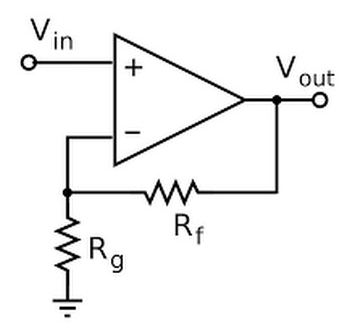
\includegraphics[width=0.25\textwidth]{media/opam-no-inversor}
		\caption{Amplificador Operacional - Configuración No Inversor}
		\label{fig:opam-no-inversor}
	\end{figure}
	
	La señal de salida mantendrá la fase de la señal viéndose afectada por la ganancia.
	
	
	\subsubsection{Amplificador Operacional Inversor}
	Configuración caracterizada por tener la señal conectada en la entrada \textbf{Inversora} o negativa del amplificador operacional.
	
	Siendo la ganancia del OPAM la que se muestra en \ref{eq:av-inversora}
	\begin{equation}
		A_v = \frac{R_f}{R_g}
		\label{eq:av-inversora}
	\end{equation}
	
	\begin{figure}[h]
		\centering
		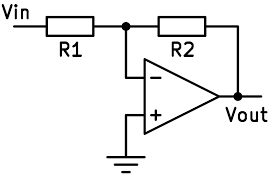
\includegraphics[width=0.3\textwidth]{media/opam-inversor}
		\caption{Amplificador Operacional - Configuración Inversosr}
		\label{fig:opam-inversor}
	\end{figure}
	
	La señal de salida se encontrará opuesta en fase en referencia a la señal de entrada viéndose afectada por el factor de ganancia.
	
	\subsubsection{Amplificador Operacional - Comparador}
	Cuando un amplificador operacional se configura como comparador, su función cambia respecto a la amplificación. En lugar de amplificar una señal de entrada, el comparador simplemente determina cuál de las dos entradas (inversora o no inversora) tiene un voltaje más alto.
	
	\begin{figure}[h]
		\centering
		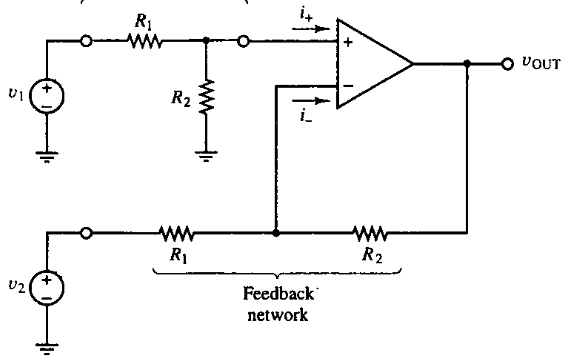
\includegraphics[width=0.4\textwidth]{media/opam-comparador}
		\caption{Amplificador Operacional - Configuración Comparador}
		\label{fig:opam-comparador}
	\end{figure}
	
	Esta configuración es útil para detectar si una señal supera cierto umbral, generando una salida digital alta o baja dependiendo de la comparación.
	
	\subsection{Servidor Web}
	Un servidor web es un sistema de software que almacena, procesa y entrega contenido web a través de internet, respondiendo a solicitudes de clientes (como navegadores) utilizando protocolos, principalmente HTTP o HTTPS. Su función es interpretar estas solicitudes, recuperar los recursos solicitados (páginas, imágenes, etc.) y entregarlos al cliente para su visualización.
	
	Una base de datos es un sistema organizado de almacenamiento de datos que permite la gestión eficiente de grandes volúmenes de información. Utiliza un modelo estructurado (relacional, documental, entre otros) para almacenar y recuperar datos de manera rápida y precisa, proporcionando mecanismos de consulta (como SQL) para acceder y manipular la información almacenada.
	
	\subsection{Base de datos}
	Una base de datos es un sistema estructurado de almacenamiento de información diseñado para gestionar, organizar y recuperar datos de manera eficiente. Utiliza un conjunto de reglas y modelos (como el modelo relacional o documental) que permite organizar la información en tablas, documentos o colecciones, facilitando el acceso y manipulación de grandes volúmenes de datos. Las bases de datos son gestionadas por sistemas de administración de bases de datos (DBMS, por sus siglas en inglés), que ofrecen mecanismos de consulta, seguridad y consistencia en el manejo de la información, permitiendo operaciones como la creación, lectura, actualización y eliminación de datos (CRUD).
	% // ================== MATERIALES Y MÉTODOS ================== //
	\section{Materiales y métodos}
	\subsection{Sensor de humedad YL-69}
	Este sensor tiene la capacidad de medir la humedad del suelo. Aplicando una pequeña tensión entre los terminales del módulo YL-69 hace pasar una corriente que depende básicamente de la resistencia que se genera en el suelo y ésta depende mucho de la humedad. Por lo tanto al aumentar la humedad la corriente crece y al bajar la corriente disminuye.
	\begin{figure}
		\centering
		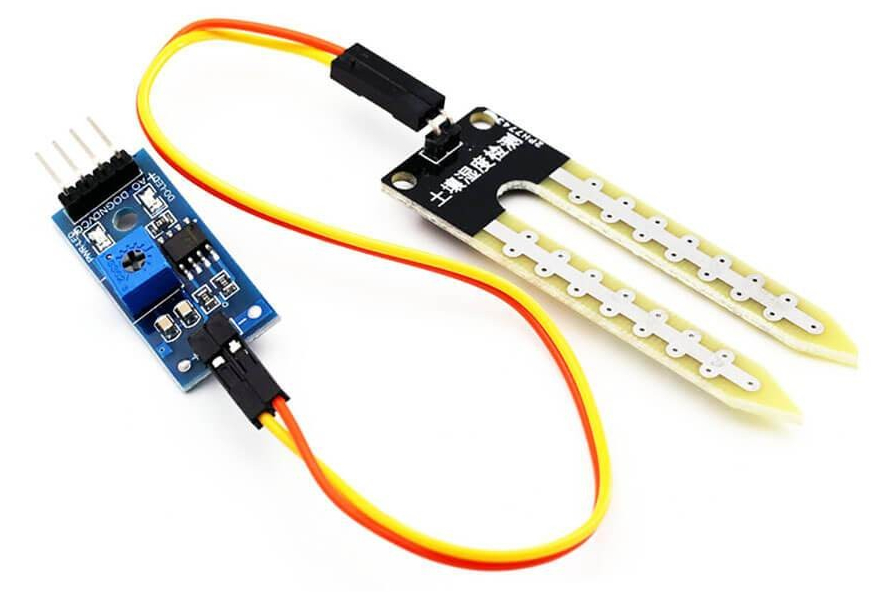
\includegraphics[width=0.4\textwidth]{media/[YL-69] YL-69 Soil Moisture Hygrometer Detection Humidity Sensor Module For arduino Development Board DIY .jpg}
		\caption{Sensor de Humedad YL-69}
		\label{fig:enter-label}
	\end{figure}
	\subsubsection{Características}
	\begin{itemize}
		\item Voltaje de operación(3.3v-5v)
		\item Modo de salida dual, salida digital y salida analógica más precisa.
		\item Dimensiones de sonda: 60mm/30mm (largo/ancho)
		\item Sensibilidad ajustable mediante potenciómetro digital.
		\item Indicadores led: alimentación (rojo) e indicador de salida de conmutación digital (verde).
		\item El módulo tiene un amplificador LM393
	\end{itemize}
	\subsubsection{Restricciones}
	\begin{itemize}
		\item Precisión limitada: No proporciona una medición altamente precisa de la humedad del suelo. 
		\item Corrosión: Las sondas están hechas de un material que puede corroerse con el tiempo debido al contacto continuo con la humedad del suelo.
		\item Interferencias en el suelo: Minerales|, sales u otros elementos en el suelo pueden afectar las lecturas, causando imprecisiones.
		\item Alcance corto: Detecta humedad solo en el área inmediata alrededor de las sondas, lo que puede no representar correctamente el estado general del suelo
		\item Consumo de energía: Mantenerlo constantemente encendido puede resultar en un consumo de energía elevado
		\item Lecturas no calibradas: No tiene una calibración interna, por lo que las lecturas pueden variar entre diferentes sensores o entornos, necesitando ajustes adicionales.
	\end{itemize}
	
	\subsection{Arduino UNO}
	El Arduino UNO es una plataforma de hardware libre basada en un microcontrolador ATmega328P. Se utiliza en el desarrollo de proyectos electrónicos y educativos debido a su simplicidad y versatilidad. Posee 14 pines digitales de entrada/salida, 6 entradas analógicas, y una interfaz USB para conectarse a la computadora. Su principal ventaja es la facilidad para programar el microcontrolador mediante el lenguaje de programación Arduino, que se basa en C/C++. El Arduino UNO es ampliamente utilizado en prototipos de automatización, robótica y control de sistemas, permitiendo a los usuarios interactuar con sensores y actuadores de forma sencilla.
	
	\begin{figure}[h]
		\centering
		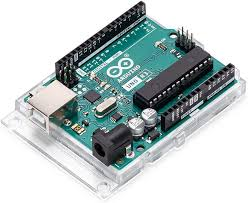
\includegraphics[width=0.3\textwidth]{media/arduino-uno.jpg}
		\caption{Arduino UNO}
		\label{fig:arduino-uno}
	\end{figure}
	
	\subsection{Raphanus Sativus}
	El Raphanus sativus, comúnmente conocido como rábano, es una planta comestible perteneciente a la familia de las Brassicaceae. Se cultiva principalmente por su raíz comestible, la cual tiene un sabor picante característico. Esta planta es rica en vitaminas, minerales, y ha sido utilizada en medicina tradicional por sus propiedades digestivas y antioxidantes. Además, el rábano juega un rol importante en la agricultura como cultivo de rotación y mejora del suelo debido a su capacidad de aflojar la tierra y suprimir malezas.
	
	\begin{figure}[h]
		\centering
		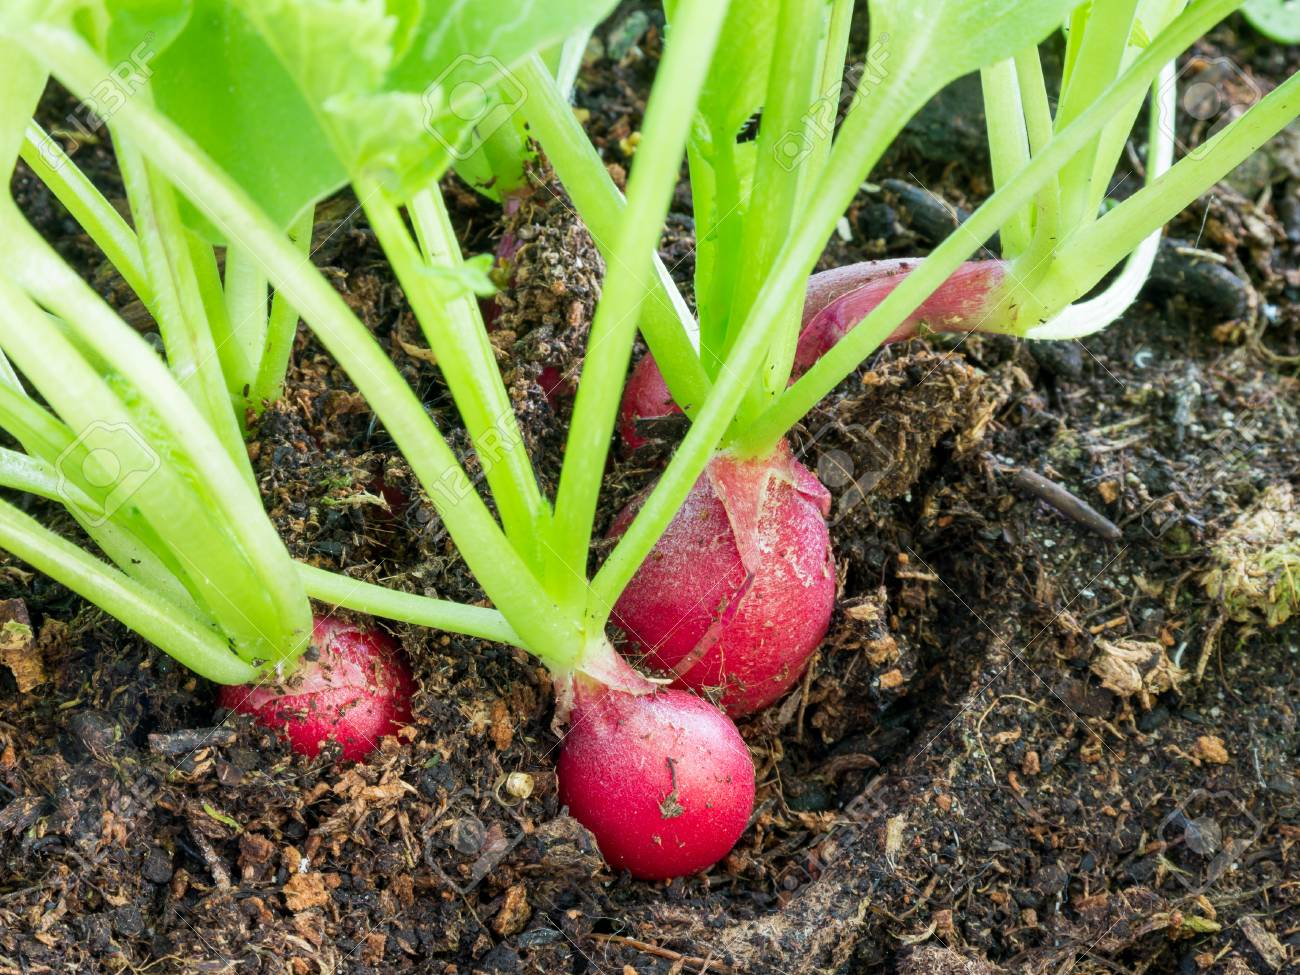
\includegraphics[width=0.4\textwidth]{media/raphanos.jpg}
		\caption{Raphanus sativus : Rabano}
		\label{fig:raphanus-sativus}
	\end{figure}
	
	
	% // ================== IMPLEMENTACIÓN ================== //
	\section{Implementación}
	
	\subsection{Amplificador Operacional en Arduino UNO Rev3}
	Las aplicaciones del amplificador diferencial se suelen aplicar en cada rama de la ingeniero electrónica desde los sistemas digitales hasta el procesamiento digital de señales se puede apreciar su influencia e importancia para este dentro del área de los microcontroladores, siendo así que este figura en partes importantes del Arduino UNO para el control en la alimentación y la otra un tanto más relevante el conversor A/D integrado dentro del ATmega328p, esta representación se puede apreciar en la figura \ref{fig:arduino-uno-esquematico}
	
	\begin{figure}[h]
		\centering
		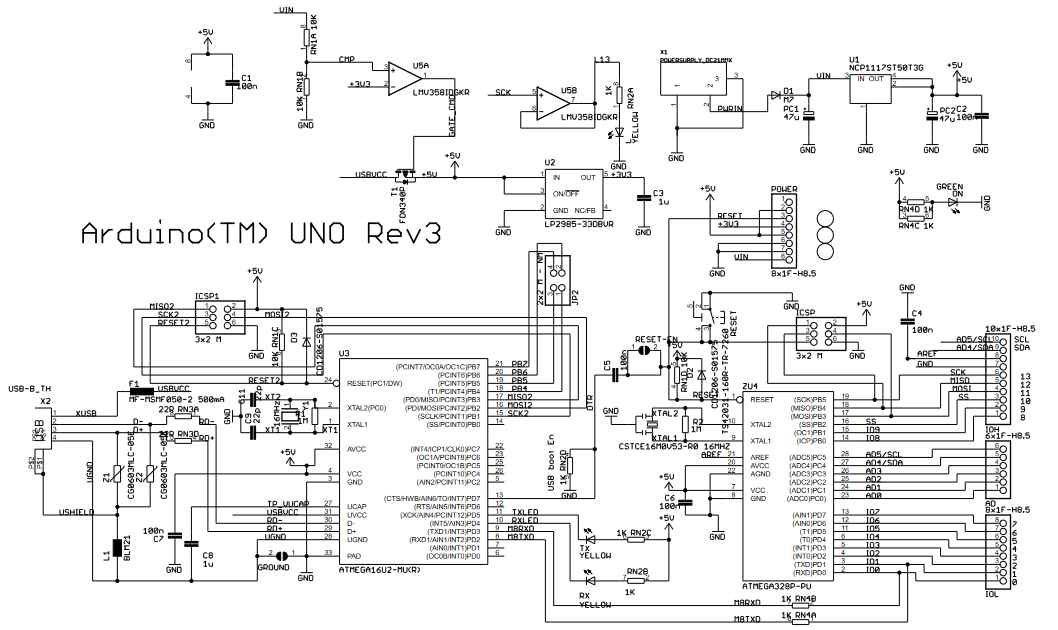
\includegraphics[width=0.5\textwidth]{media/arduino-uno-esquema}
		\caption{Circuito esquemático - Arduino UNO Rev3}
		\label{fig:arduino-uno-esquematico}
	\end{figure}
	
	Para que el amplificador operacional pueda controlar la fuente de alimentación fue configurado como comparador de voltajes y mediante el cual se indica si Arduino UNO esta siendo alimentado por su entrada $V_in$ o mediante una conexión USB.
	
	Esta comportamiento se define gracias al juego de resistencias y salida mediante un diodo led para el amplificador U5B, el cual se encarga de gestionar la energía para un funcionamiento adecuado.
	
	Como se menciono previamente los amplificadores operacionales también se encargan de otra parte muy importante esta vez centrada en el procesamiento de datos y la cual consiste en la conversión de los datos analógicos a digitales, en este apartado este dispositivo electrónico trabaja en conjunto a otras etapas para poder amplificar, tomar una muestra, comparar con una señal de referencia para finalmente convertir el resultado a un número binario en relación con la amplitud de la señal analógica.
		
	\subsection{Microcontralador ATMEGA328p}
	Para realizar el acondicionamiento de la señal se hizo uso del microcontrolador Arduino UNO Rev3 el cual a su vez depende del ATmega328 para el procesamiento, control y respuesta para una determinada entrada, este microcontrolador esta compuesto por diferentes etapas o bloques que se aprecian en la figura \ref{fig:esquema-atmega328} el bloque A/D (Convertidor Analógico - Digital) de 10 bits la parte central de este estudio y mediante el cual se realizará el filtrado de la señal de ruido facilitando el acondicionando de la señal del entrada del sensor de humedad YL-69.
	
	\begin{figure}[h]
		\centering
		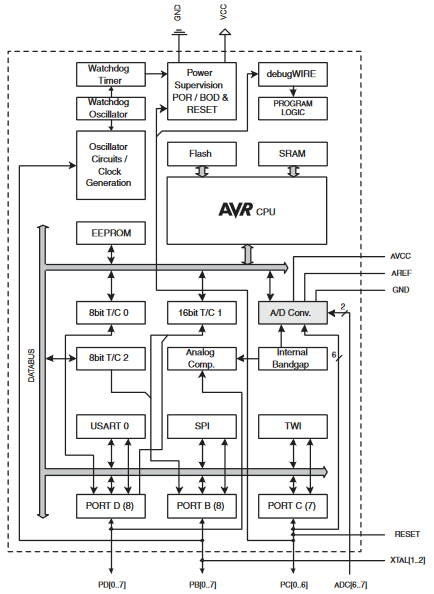
\includegraphics[width=0.5\textwidth]{media/esquema-atmega328}
		\caption{Diagrama de Bloques - ATmega328}
		\label{fig:esquema-atmega328}
	\end{figure}
	
	\subsection{Conversor Analógico Digital}
	Un conversor analógico-digital (ADC, por sus siglas en inglés) es un dispositivo que convierte una señal analógica (un voltaje continuo) en una señal digital (un número discreto que representa el nivel de la señal analógica). En el diseño de muchos ADCs, se incluyen amplificadores operacionales como componentes clave para mejorar la precisión y exactitud de la conversión. A continuación, te explico su funcionamiento detallado en función del amplificador operacional y te presento un diagrama de bloques típico.
	
	\subsection{Muestreo doble correlacionado}
	La técnica de muestreo doble correlacionado se utiliza en el acondicionamiento de señales, particularmente en aplicaciones donde se requiere extraer una señal de bajo nivel inmersa en ruido. Consiste en realizar dos etapas de muestreo correlacionado (una detrás de otra para una diferencia de tiempo mínima).
	
	En el muestreo doble correlacionado se tiene la señal de muestra en la cual se recupera una muestra de la señal con el ruido adicional y una segunda (señal de referencia) en la cual solo se trata de capturar el ruido de la señal siendo así que al aplicar la diferencia entre ambas se pueda eliminar/filtrar el ruido.
	
	Esto se puede ejemplificar en la ecuación \ref{eq:mdc}
	
	\begin{align}
		C_o &= V_m + V_r - V_r \\
		\label{eq:mdc}
		C_o &= V_m
	\end{align}
	Donde:\\
	$C_o$: Señal de salida correlacionada\\
	$V_m$: Señal de muestreo \\
	$V_r$: Señal de ruido\\
	
	\subsection{Implementación en Arduino}
	
	Para la implementación a nivel lógico se hizo uso del entorno Arduino IDE 2.3.0 la cual es un entorno gráfico para el desarrollo de aplicaciones en hardware mediante arduino, el código definido se dividió en 3 partes principales.
	
	\begin{itemize}
		\item Variables
		\item Función setup()
		\item Función loop()
	\end{itemize}
	
	En la primera parte se describieron las variables de trabajo para la medición de humedad mediante el sensor mediante el filtro correlacionado y sin el, así como la constante de tiempo (en milisegundos) para el muestreo de señal de ruido.
	
	\begin{lstlisting}[caption=Arduino Muestreo doble Correlacionado, numbers=none, label=cd:codigo-mdc]
		// CONSTANTES
		const float TIEMPO_MUESTREO = 1;
		
		// VARIABLES
		int humedad, humedadPorcentual;
		int humedadFiltro, muestraFiltro, humedadPorcentualFiltro, correlacion;
		
		void setup() {
			// Iniciar la comunicacion serial
			Serial.begin(9600);
		}
		
		void loop() {
			// Sensado sin filtro
			humedad = analogRead(A0); // Salida en bits
			humedadPorcentual = map(humedad, 0, 1023, 100, 0); // Salida porcentual analogica
			Serial.print("Humedad SF: ");
			Serial.println(humedad);
			
			// Sensando mediante el algoritmo de muestreo doble correlacionado
			humedadFiltro = analogRead(A1); // Salida en bits
			delayMicroseconds(TIEMPO_MUESTREO);
			muestraFiltro = analogRead(A1);
			
			// Filtrado de la senal
			correlacion = humedadFiltro - abs(humedadFiltro - muestraFiltro);
			humedadPorcentualFiltro = map(correlacion, 0, 1023, 100, 0);
			
			Serial.print("Humedad MDC: ");
			Serial.println(correlacion);
			
			delay(3000);
		}
	\end{lstlisting}
	 
	En el código definido en el bloque \ref{cd:codigo-mdc} la parte central y filtrado de la señal se encuentra dentro de la función \textbf{loop()} la cual toma una muestra de la señal del sensor y su respectiva referencia 1 milisegundo después para después realizar la diferencia de estas señales, sin embargo en el código antes propuesto el algoritmo de correlación  se vio modificado debido a que la diferencia para el tiempo de muestreo para la señal de referencia recupera casi el mismo valor que la señal de muestra, siendo así que la diferencia será el valor de ruido, es por ello que para obtener una señal de correlación adecuada primer se obtiene el valor del ruido y este se resta a la señal de referencia original, esto se puede apreciar en el listing \ref{cd:mdc-modificado}
	
	\begin{lstlisting}[caption=Arduino Muestreo doble Correlacionado, numbers=none, label=cd:mdc-modificado]
		void loop() {
			
			// Sensando mediante el algoritmo de muestreo doble correlacionado
			humedadFiltro = analogRead(A1); // Salida en bits
			delayMicroseconds(TIEMPO_MUESTREO);
			muestraFiltro = analogRead(A1);
			
			// Filtrado de la senal
			correlacion = humedadFiltro - abs(humedadFiltro - muestraFiltro);
			humedadPorcentualFiltro = map(correlacion, 0, 1023, 100, 0);
			
		}
	\end{lstlisting}
	
	% // ================== CULTIVOS  ================== //
	\section{Cultivo del Rhapanus Sativus}
	\subsection{Preparación de la Maceta y el Sustrato}
	Para la siembra del rabanito, emplearemos una maceta de polipropileno de 15 $cm^2$. Se adecuó el envase de modo que tenga un correcto drenaje y se agregó tierra rica en nutrientes para favorecer el crecimiento de las plántulas.
	\subsection{ Siembra de Rábanos}
	Se emplearon alrededor de 50 semillas de rábano, sembradas en el envase de polipropileno previamente preparado. Aproximadamente 30 de ellas germinaron en los primeros 5 días. A los diez días de la siembra, comenzaron a aparecer las primeras hojas verdaderas en las plantas.
	Para el análisis, se seleccionaron ocho plántulas de 3 cm de altura, distribuidas en el envase a una distancia de 5 cm entre cada una, con el objetivo de asegurar un crecimiento uniforme y adecuado espacio para cada plántula.
	
	\begin{figure}[h]
		\centering
		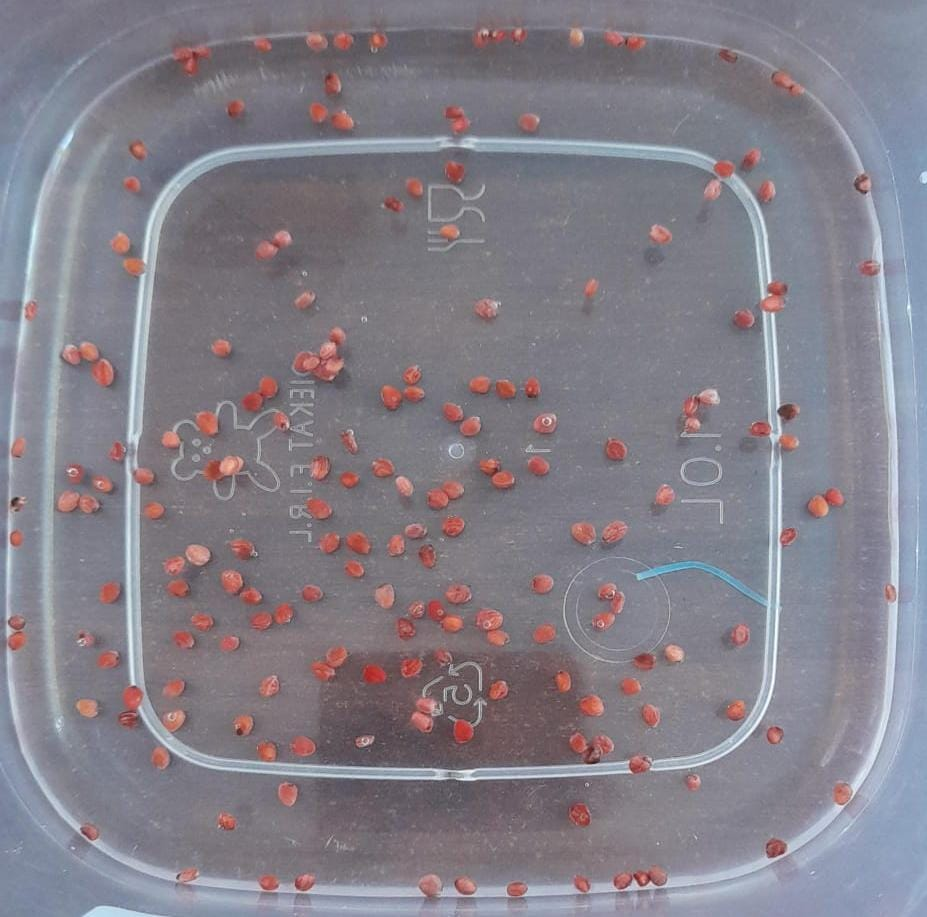
\includegraphics[width=0.35\textwidth]{media/Semillas.jpg}
		\caption{Semillas de Raphanus Sativus en preparación para ser plantadas}
		\label{fig:raphanus-semillas}
	\end{figure}
	
	\begin{figure}[h]
		\centering
		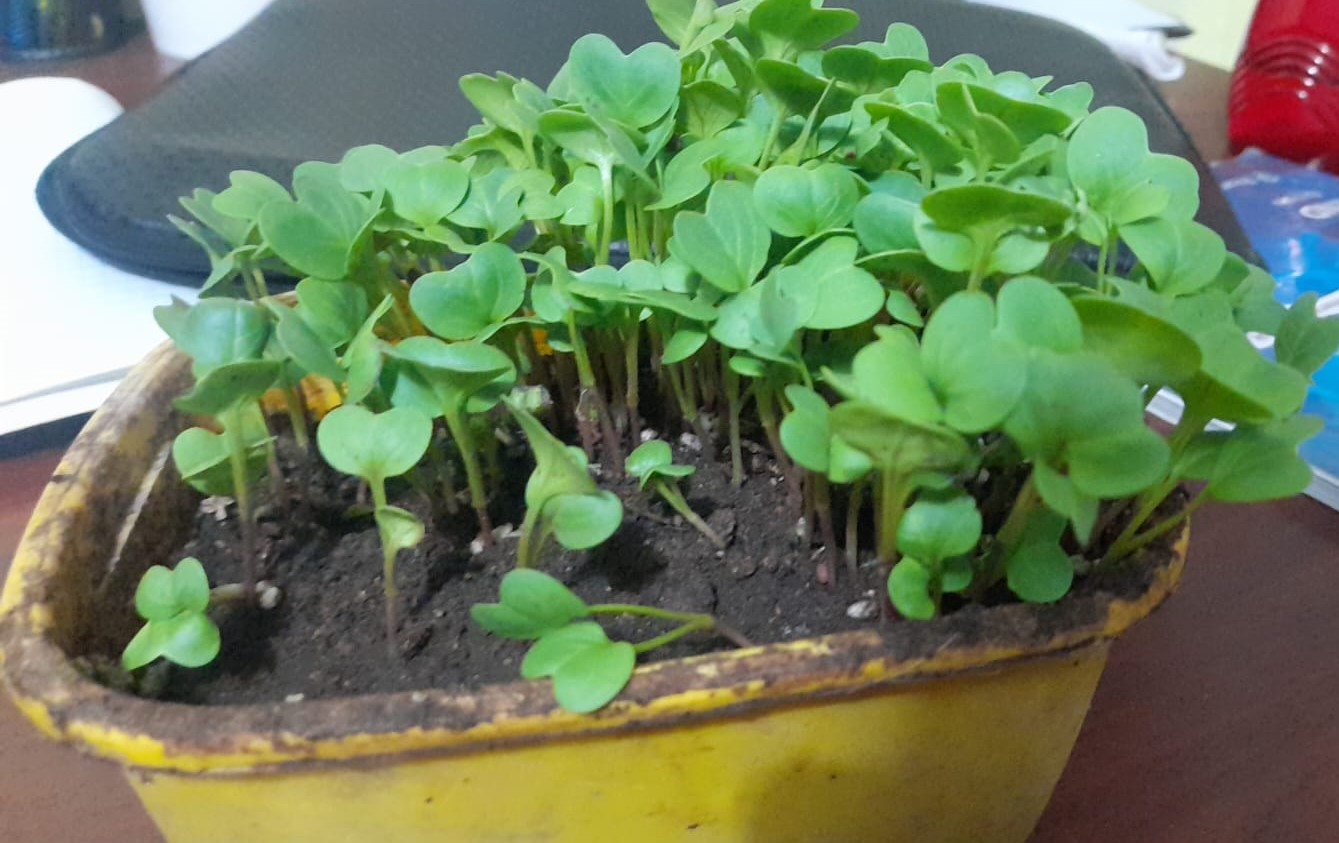
\includegraphics[width=0.4\textwidth]{media/Dia 5.jpg}
		\caption{Crecimiento de la planta al quinto día}
		\label{fig:raphanus-dia5}
	\end{figure}
	
	\begin{figure}[h]
		\centering
		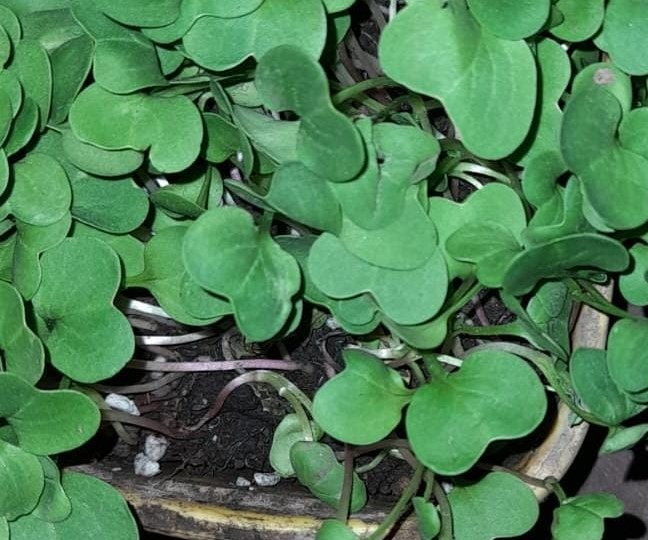
\includegraphics[width=0.4\textwidth]{media/Dia 10.jpg}
		\caption{Crecimiento de la planta al décimo día}
		\label{fig:raphanus-dia10}
	\end{figure}
	
	\begin{figure}[h]
		\centering
		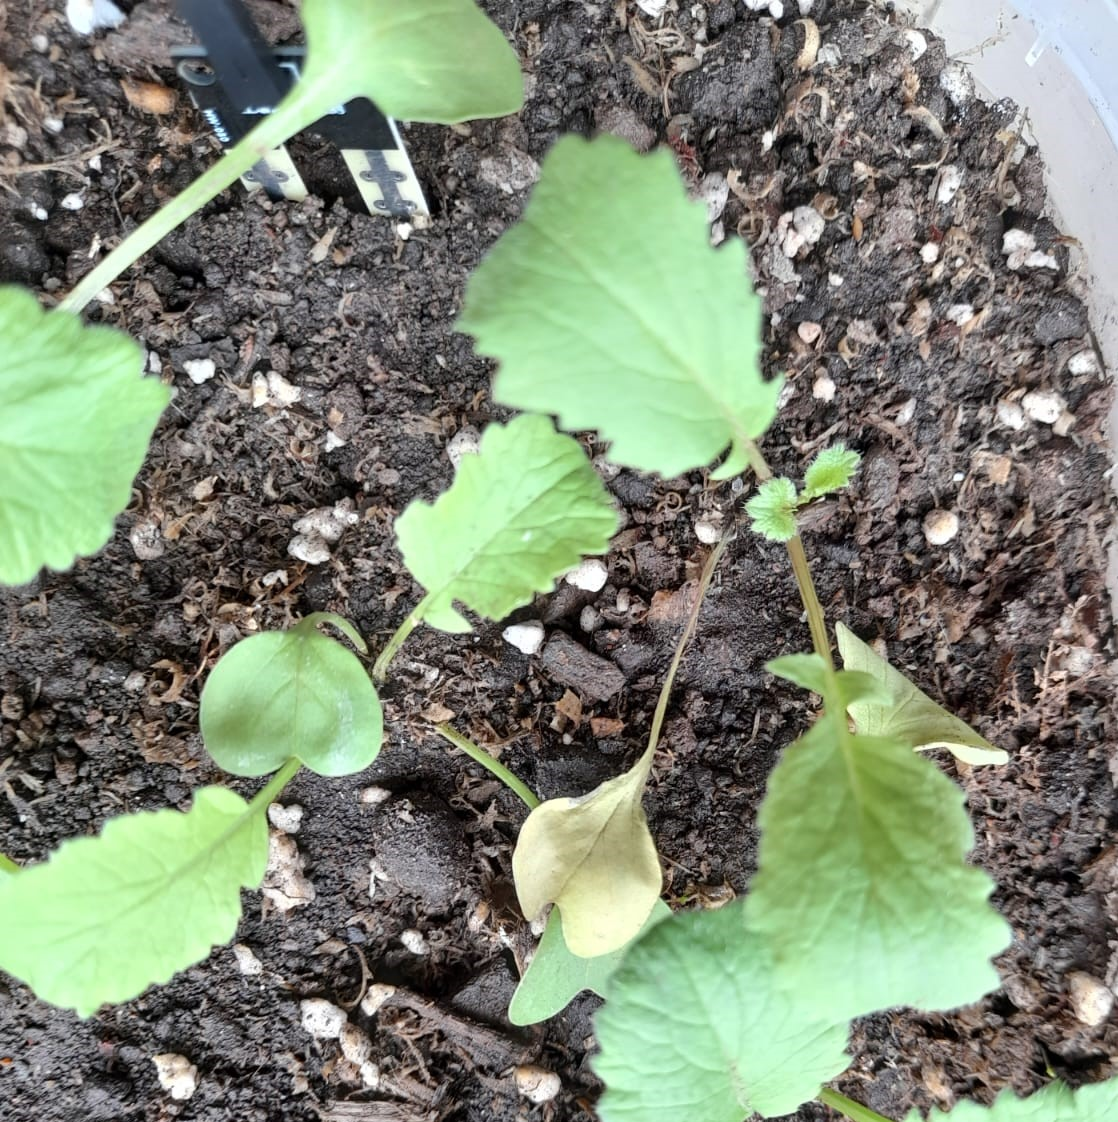
\includegraphics[width=0.5\linewidth]{media/Dia 15 .jpg}
		\caption{Crecimiento de la planta al quinceavo día}
		\label{fig:raphanus-dia15}
	\end{figure}
	
	\subsection{Monitoreo de Humedad en el Sustrato}
	En el nuevo envase, se colocaron los sensores de humedad a una distancia de 10 cm entre ellos. Esta medida fue recomendada para obtener lecturas similares, especialmente en sustratos homogéneos, ya que ayuda a lograr una medición uniforme de la humedad en el área.
	Las lecturas de los sensores se registraron cada 5 días. A continuación, se presenta un cuadro con los datos registrados en el monitoreo:
	
	De acuerdo a algunos datos el porcentaje sugerido de humedad para la planta varía entre 60\% y 80 \%, de acuerdo a ello, la planta era regada cada 2 días manteniendo el porcentaje sugerido.
	
	\begin{table}[]
		\centering
		\begin{tabular}{|c|c|c|c|}
			\hline
			\textbf{Fechas} & \textbf{Acción}     & \textbf{Humedad S1} & \textbf{Humedad S2} \\ \hline
			15 de Octubre   & Siembra             & 51\%                & 49\%                \\ \hline
			20 de Octubre   & Primeras Hojas      & 60\%                & 57\%                \\ \hline
			25 de Octubre   & Hojas Desarrolladas & 81\%                & 79\%                \\ \hline
			30 de Octubre   & Plantula 5CM        & 80\%                & 76\%                \\ \hline
		\end{tabular}
	\end{table}
	
	\subsection{Observación del Crecimiento}
	Como se mencionó, las plantas de rabanito requieren un nivel de humedad en el rango de 60\% a 80\% para garantizar un buen desarrollo. Este nivel es fundamental para que la planta crezca de manera óptima y produzca rabanitos de sabor agradable.
	
	Según algunos estudios, cuando la humedad es insuficiente, la planta no se desarrolla de manera eficiente y los rabanitos tienden a presentar un sabor más agrio y desagradable, lo que disminuye su calidad.
	
	\begin{figure}[h]
		\centering
		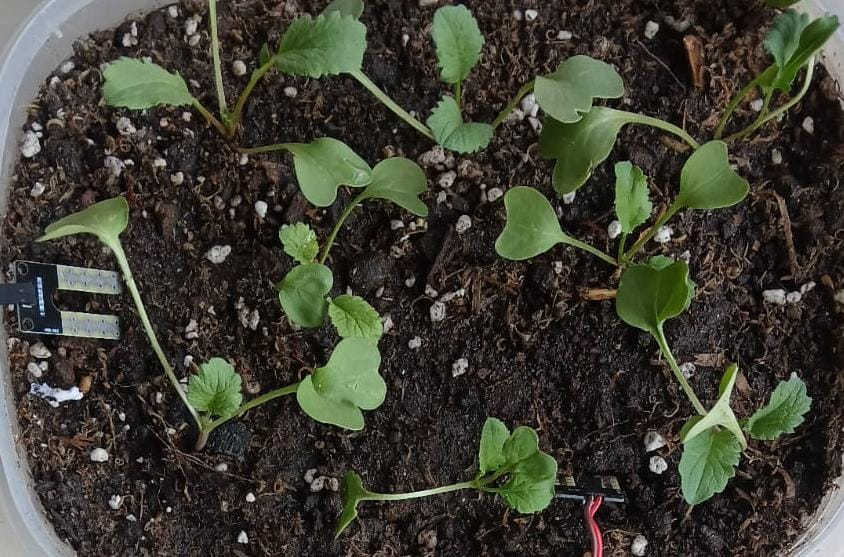
\includegraphics[width=0.35\textwidth]{media/Opt 15.jpg}
		\caption{Raphanus Sativus entre el 60\% y 80\%}
		\label{fig:raphanus-humedad-optima}
	\end{figure}
	En el día 15, se observó que algunas plántulas murieron debido al exceso de agua, ya que la humedad superaba el rango establecido. 
	\begin{figure}[h]
		\centering
		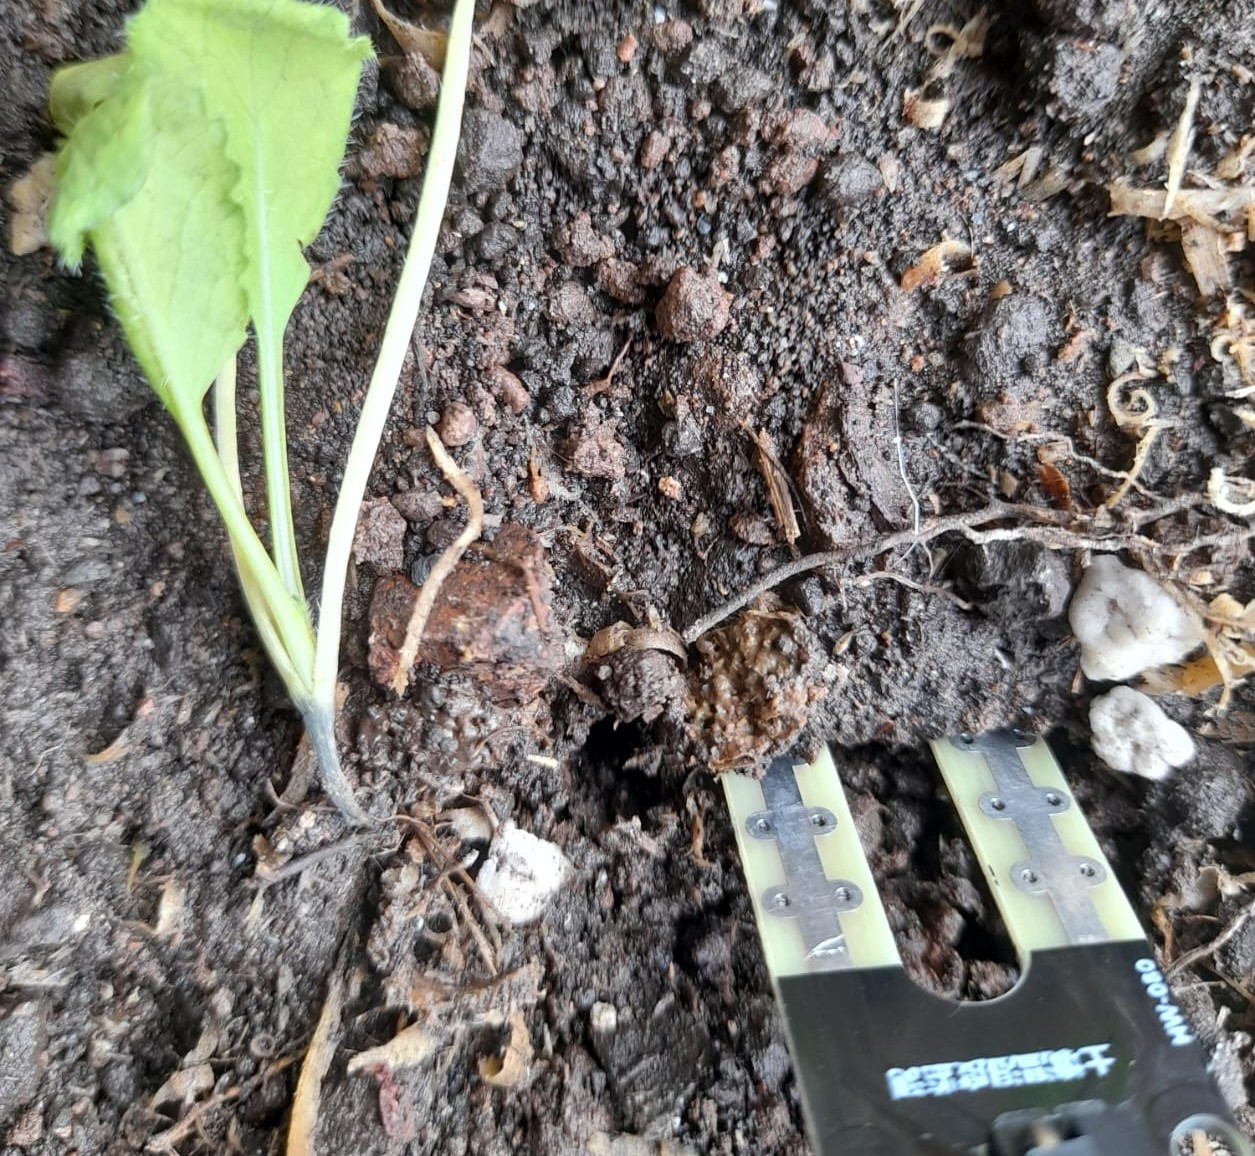
\includegraphics[width=0.35\textwidth]{media/H_Mayor.jpg}
		\caption{Raphanus Sativus con una humedad superior 80\%}
		\label{fig:raphanus-humedad-excesiva}
	\end{figure}
	
	
	
	\bibliographystyle{IEEEtran}
	\bibliography{biblio}
\end{document}